%!TEX root = main.tex




\section{Our Construction} 
\label{sec:construction}
\label{sec:random-bin-assignment}

We first present the oblivious random bin assignment algorithm (Section~\ref{sec:obin})  and then use it to implement our bucket oblivious random permutation (Section~\ref{sec:ORP}) and bucket oblivious sort (Section~\ref{sec:osort}).

\newcommand{\val}{{\sf value}}
\newcommand{\pref}{{\sf pref}}

\begin{figure*}[h!]
\centering

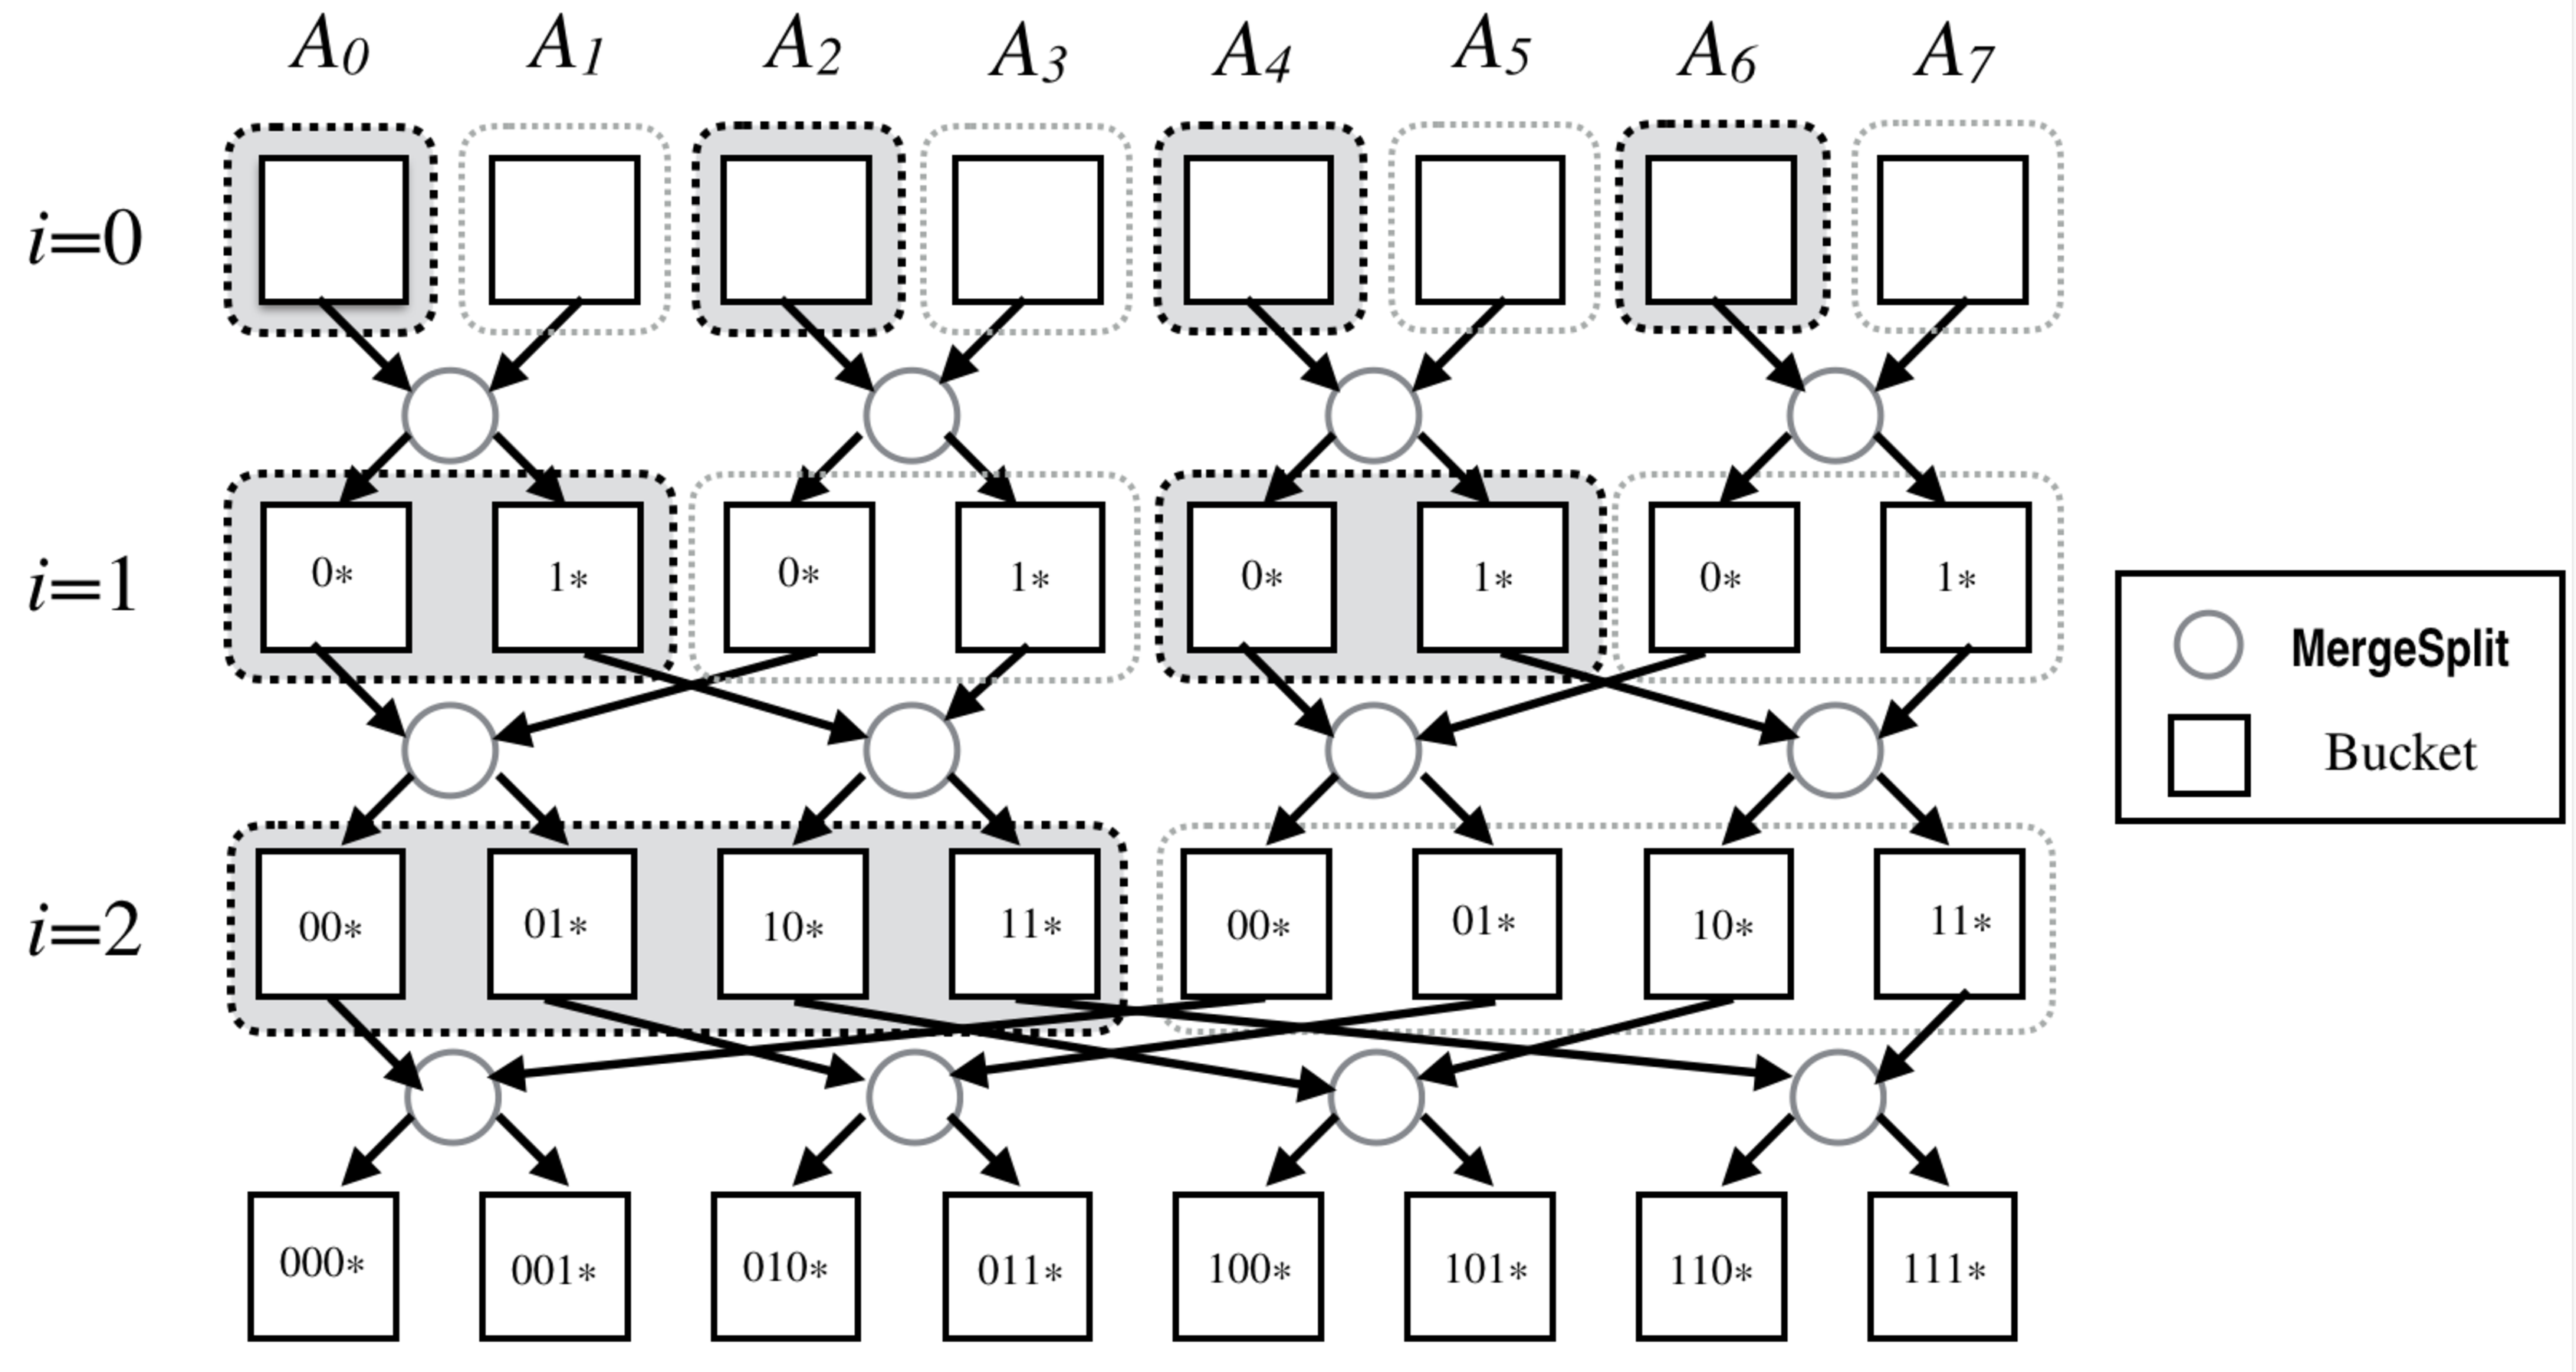
\includegraphics[width=0.75\textwidth]{RadixBucketSort1.pdf}
\captionof{figure}{Oblivious random bin assignment with 8 buckets.}
%The \textsc{MergeSplit} procedure takes elements from two buckets at level $i$ and put them into two buckets at level $i+1$, according to the $(i+1)$-th most significant bit of the keys. 
%At level $i$, every $2^{i}$ consecutive buckets are semi-sorted by the most significant $i$ bits of the keys.
\label{fig:radix-sort}

\bigskip
\begin{algorithm}[Oblivious Random Bin Assignment]
\begin{algorithmic}
\State
\State \textbf{Input}: an array $\X$ of size $n$
\State Choose a bucket size $Z$ and let $B$ be the smallest power of two that is $\geq 2n/Z$. 
\State Define $(\log B+1)$ arrays, each containing $B$ buckets of size $Z$. Denote the $j$-th bucket of the $i$-th array $A_j^{(i)}$.
\State For each element in $\X$, assign a uniformly random key in $[0,B-1]$.
\State Evenly divide $\X$ into $B$ groups. Put the $j$-th group into $A_j^{(0)}$ and pad with dummy elements to have size $Z$.

\For {$i=0,\ldots,\log B-1$}
    \For {$j=0,\ldots,B/2$}
        \State $(A^{(i+1)}_{2j}, A^{(i+1)}_{2j+1}) \leftarrow \textsc{MergeSplit}(A^{(i)}_{j'+j}, A^{(i)}_{j'+j+2^i}, i)$ where $j'=\lfloor j / {2^i} \rfloor \cdot 2^{i+1}$
        \State \Comment{Input: $j$-th pair of buckets with distance $2^i$ in $A^{(i)}$; Output: $j$-th pair of buckets in $A^{(i+1)}$}
        %\State Let $(A_0, A_1$) be the $j$-th pair of buckets with distance $2^i$ in $A^{(i)}$ 
        %\State Let $(A'_0, A'_1)$ be the $j$-th pair of buckets in $A^{(i+1)}$
        %\State $(A'_0, A'_1) \leftarrow \textsc{MergeSplit}(A_0, A_1, i)$ 
        
    \EndFor
\EndFor    
\State \textbf{Output:} $A^{(\log B)}$

\medskip
\Function{$(A'_0, A'_1) \leftarrow$ MergeSplit}{$A_0, A_1, i$}
    \State $A'_0$ receives all real elements in $A_0 \cup A_1$ where the $(i+1)$-st MSB of the key is $0$   
    \State $A'_1$ receives all real elements in $A_0 \cup A_1$ where the $(i+1)$-st MSB of the key is $1$
    \State If either $A'_0$ or $A'_1$ receives more than $Z$ real elements, the procedure aborts with {\sf overflow}
    \State Pad $A'_0$ and $A'_1$ to size $Z$ with dummy elements and return $(A'_0, A'_1)$
\EndFunction   
\end{algorithmic}
\label{code:obin}
\end{algorithm}

\bigskip
%\begin{table*}[t]
\centering
\begin{tabular}{|c|c|c|c|c|}
    \hline
    Algorithm & Oblivious & Client storage & Runtime & Error probability \\
    \hline
    merge sort & no & $O(1)$ & $2n \log n$ & 0 \\
    Bitonic sort & yes & $O(1)$ & $n\log^2 n$ & 0 \\
    AKS sort & yes & $O(1)$ & $5.4\times10^7 \times n\log n$ & 0 \\
    Zigzag sort & yes & $O(1)$ & $8\times10^4 \times n\log n$ & 0 \\
    Randomized Shellsort & yes & $O(1)$ & $24n\log n$ & $\approx n^{-3}$ \\
    \hline
    \textbf{Bucket oblivious sort} & yes & $2Z$ & $6 n\log n$ & $\approx e^{-6/3}$\\
    \textbf{Bucket oblivious sort} & yes & $O(1)$ & $2n\log n \log^2 Z$ & $\approx e^{-6/3}$ \\
    \hline   
\end{tabular}
\captionof{table}{Runtime of bucket oblivious sort and classic non-oblivious and oblivious sort algorithms.}
\label{tab:compare}
%\end{table*}

\end{figure*}
\subsection{Oblivious Random Bin Assignment.}
\label{sec:obin}

The input to the oblivious random bin assignment algorithm is an array $\X$ of $n$ elements. 
The goal is to obliviously and uniformly randomly distribute the elements into a set of bins. Each element is assigned to independent random bin, and elements are then routed into the bins obliviously. 

The algorithm first chooses a bucket size $Z$, which can be set to the security parameter $\sec$. 
Then, it constructs $B=\lceil 2n/Z \rceil$ buckets each of size $Z$.
Without loss of generality, assume $B$ is a power of $2$ --- if not, pad it to the next power of 2. Note that the algorithm introduces $n$ dummy elements, and the output is twice the size of the input array. %If needed, see Appendix~\ref{appx:formal} for a formal definition of the functionality. 

%also assume elements in $\X$ are distinct --- if not, we can use the indices of the elements within $\X$ to break ties.

Figure~\ref{fig:radix-sort} gives a graphic illustration of the algorithm for 8 input buckets and Algorithm~\ref{code:obin} gives the pseudocode.
Each element in $\X$ is assigned a random key in $[0, B-1]$ which represents a destination bucket.
Next, the algorithm repeatedly calls the \textsc{MergeSplit} subroutine to exchange elements between bucket pairs in $\log B$ levels to distribute elements into their destination buckets. 
The operation $(A'_0,A'_1)\leftarrow \textsc{MergeSplit}(A_0,A_1,i)$ involves four buckets at the time, distributing the elements in the two input buckets $A_0$ and $A_1$ into two output buckets $A'_0$ and $A'_1$.
$A'_0$ receives all the keys with $(i+1)$-th most significant bit (MSB) as 0 and $A'_1$ receives all the keys with $(i+1)$-th MSB as 1.


For now, assume the client can locally store two buckets.
For each \textsc{MergeSplit}, it reads (and decrypts) the two input buckets, swaps elements in the two buckets according to the above rule, and writes to the two output buckets (after re-encryption).
It is then easy to see that Algorithm~\ref{code:obin} is oblivious since the order in which the client reads and writes the buckets is fixed and independent of the input array.
%We discuss how to extend the algorithm to work with $O(1)$ client storage in Section~\ref{sec:O1client}. 

When no bucket overflows, all real elements are correctly put into their assigned bins.
We now show that the probability of overflow is exponentially small in $Z$. 
Intuitively, this is because each bucket contains (in expectation) half dummy elements that serve as a form of ``slack'' to disallow overflow.

\begin{lemma}
\label{lemma:shuffle}
Overflow happens with at most $\epsilon(n, Z) = 2n/Z \cdot \log(2n/Z) \cdot e^{-Z/6}$ probability.
\end{lemma}
\begin{proof}
\label{clm:proof-shuffle}
Consider a bucket $A^{(i)}_b$ at level $i$.
%Let $T$ be the set of real elements. For $t \in T$, $i \in \{1,\ldots,\log B\}$ and $b \in [B]$, let $X_{i,b}^{t}$ be the indicator random variable that $t$ is assigned to bucket $A^{(i)}_b$.
%$X_{i,b}=\sum_{t \in T}X_{i,b}^{t}$ denotes the load of $A^{(i)}_b$. 
Observe that this bucket can receive real elements from $2^i$ initial buckets, each containing $Z/2$ real elements.
For each such element, we have chosen an independent and uniformly random key;
the element reaches $A^{(i)}_b$ only when the most significant $i$ bits of its key match $b$,
which happens with exactly $2^{-i}$ probability.
A Chernoff bound shows that $A^{(i)}_b$ overflows with less than $e^{-Z/6}$ probability.
Hence, a union bound over all levels and all buckets 
shows that overflow happens with less than $B \cdot \log B \cdot e^{-Z/6} = \epsilon(n,Z)$ probability.
\end{proof}

%In Appendix~\ref{appx:formal} we formally describe the ideal functionality of oblivious random bin assignment, and show that the above describe algorithm obliviously implements this functionality. 

\subsection{Bucket Oblivious Random Permutation.}
\label{sec:ORP}

After performing the oblivious random bin assignment, ORP can be simply achieved as follows:
scan the array and delete dummy elements from each bin (note that within each bin it is guaranteed that the real elements appear before the dummy elements). Then obliviously permute each bin and finally concatenate all bins.  We have:

%The ORP reveals the loads of the output buckets of bin assignment, that is, the number of real elements in each bucket. 

\begin{lemma}
Bucket ORP oblivious implement the permutation functionality except for $\e(n,Z)$ probability. 
\end{lemma}

\begin{proof}
We first describe the simulator. 
The access pattern of the oblivious bin assignment algorithm is deterministic and the same for every input, where the overflow even is independent of the input itself. Therefore, it is easy to simulate the bin assignment. 
The simulator then pretends to simulate the randomly permuting of each bin. 
Then, 
the simulator chooses random loads $\vec{k}=(k_0, k_1, \ldots, k_{B-1})$, where $k_i$ is the load of the real elements in the $i$th bin. This is done by simply throwing $n$ elements into $B$ bins (``in the head''). If there is some $i$ for which $k_i > Z$ then the simulator aborts. The removal of the dummy elements is equivalent to the revealing of these loads. 

Clearly, $\vec{k}$ are distributed the same as in the real execution. The only difference between the simulated access pattern and the real one is in the case where the algorithm aborts as a result of an overflow before the last level, which occurs with at most $\e(n,Z)$ probability. 

We next show that the output of the algorithm is a random permutation, conditioned of the access pattern. As we previously described, it is actually enough to condition on the vector of random loads $\vec{k}=(k_0, k_1, \ldots, k_{B-1})$. We show that given any such vector, all permutations are possible.  

Fix a particular load $\vec{k}=(k_0, k_1, \ldots, k_{B-1})$. The algorithm works by first assigning the real elements into the bins, and then permuting within each bin. For every input, there are exactly ${n \choose k_0,\ldots,k_{B-1}}$ ways to distribute the real elements into the bins while achieving the vector of loads $\vec{k}$. Then, each bin is individually permuted, i.e., within each bin $i$, we have $k_i$ different possible ordering. Overall, 
the total number of possible outputs with that load is then
\[{n \choose k_0,\ldots,k_{B-1}} \cdot k_0! \cdot \ldots \cdot k_{B-1}! = n!\]
That is, even conditioned on some specific loads $\vec{k}=(k_0, k_1, \ldots, k_{B-1})$, all permutations are still possible.
Therefore, for every $\pi$, $\Pr\left[\Pi = \pi \mid \vec{K}=\vec{k} \right] = \frac 1 {n!}$, and
\[ \Pr\left[\Pi = \pi\right] = \sum_{\vec{k}} \Pr\left[\Pi = \pi \mid \vec{K}=\vec{k} \right] \cdot \Pr\left[\vec{K}=\vec{k}\right] = \frac {1}{n!} \]
%&= \frac {1}{n!} \cdot \sum_{\vec{k}} \Pr\left[\vec{K}=\vec{k}\right] = \frac {1}{n!}

The ORP fails only when some bin overflows during the oblivious random bin assignment, which happens with $\epsilon(n,Z)$ probability by Lemma~\ref{lemma:shuffle}.
\end{proof}

\subsection{Bucket Oblivious Sort.}
\label{sec:osort}
Once we have ORP, it is easy to achieve oblivious sort: just invoke any non-oblivious comparison-based sort after ORP.

Since the functionality is deterministic, it is enough to consider separately correctness and simulation. Correctness follows from directly from the correctness of the ORP and the non-oblivious sort. As for obliviousness, given any input array, one can easily simulate the algorithm by first randomly permuting the array and then running the comparison-based non-oblivious sort. 
The access patterns of a comparison-based sort depend only on the relative ranking of the input elements, which is independent of the input array once the array has been randomly permuted. 

\subsection{Efficiency.}
\label{sec:efficiency}

We analyze the efficiency of our algorithms and compare them to classic non-oblivious oblivious sorting algorithms in Table~\ref{tab:compare}.
We measure runtime using the number of memory accesses the clients needs to perform on the server.



% Merge sort, a well known non-oblivious sort, runs in $2n\log n$ time. 
% It has in $\log n$ stages; each stage merges smaller sorted subarrays into larger sorted subarrays,
% which reads and writes the entire array in the process.
% Bitonic sort uses $\frac 14 n\log^2 n$ comparisons.
% According to~\cite{zigzag}, the AKS sorting network has $13613047 n\log n$ comparisons and the Zigzag sort uses $19600n\log n$ comparisons (with best known explicit constructions). 
% Randomized Shellsort~\cite{RandShellsort} needs $6n\log n$ comparisons (there are $\log n$ iterations, six passes per iteration, and $n$ comparisons per pass). 
% The number of memory accesses is four times of the number of
% comparisons for Bitonic, AKS, Zigzag, and randomized Shellsort.


For our algorithms, assuming the client can store $2Z$ elements locally, each $2n$-sized array is read and written once and there are $\log(2n/Z)<\log n$ of them.
So oblivious bin assignment and bucket ORP run in (less than) $4n\log n$ time.
Note that the last step of ORP, i.e., permuting each output bucket, can be incorporated with the last level of oblivious bin assignment.
Bucket oblivious sort additionally invokes a non-oblivious sort, and thus runs in $6n\log n$ time. 
This is within $3\times$ of merge sort and beats bitonic sort when $n$ is moderately large;
for example, $5\times$ faster than bitonic for $n=2^{30}$.
For an overflow probability of $2^{-80}$ and most reasonable values of $n$, $Z = 512$ suffices. 


%%% Local Variables:
%%% mode: latex
%%% TeX-master: "main"
%%% End:
